\documentclass[14pt]{extbook}
\usepackage{multicol, enumerate, enumitem, hyperref, color, soul, setspace, parskip, fancyhdr} %General Packages
\usepackage{amssymb, amsthm, amsmath, bbm, latexsym, units, mathtools} %Math Packages
\everymath{\displaystyle} %All math in Display Style
% Packages with additional options
\usepackage[headsep=0.5cm,headheight=12pt, left=1 in,right= 1 in,top= 1 in,bottom= 1 in]{geometry}
\usepackage[usenames,dvipsnames]{xcolor}
\usepackage{dashrule}  % Package to use the command below to create lines between items
\newcommand{\litem}[1]{\item#1\hspace*{-1cm}\rule{\textwidth}{0.4pt}}
\pagestyle{fancy}
\lhead{Progress Quiz 10}
\chead{}
\rhead{Version C}
\lfoot{6232-9639}
\cfoot{}
\rfoot{Fall 2020}
\begin{document}

\begin{enumerate}
\litem{
Write the equation of the graph presented below in the form $f(x)=ax^2+bx+c$, assuming  $a=1$ or $a=-1$. Then, choose the intervals that $a, b,$ and $c$ belong to.
\begin{center}
    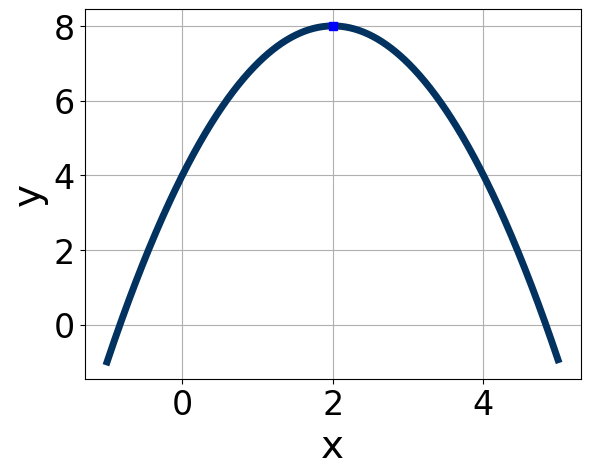
\includegraphics[width=0.5\textwidth]{../Figures/quadraticGraphToEquationC.png}
\end{center}
\begin{enumerate}[label=\Alph*.]
\item \( a \in [-2, 0], \hspace*{5mm} b \in [3, 6], \text{ and } \hspace*{5mm} c \in [2, 10] \)
\item \( a \in [0, 3], \hspace*{5mm} b \in [-8, -3], \text{ and } \hspace*{5mm} c \in [11, 15] \)
\item \( a \in [-2, 0], \hspace*{5mm} b \in [-8, -3], \text{ and } \hspace*{5mm} c \in [2, 10] \)
\item \( a \in [0, 3], \hspace*{5mm} b \in [3, 6], \text{ and } \hspace*{5mm} c \in [11, 15] \)
\item \( a \in [-2, 0], \hspace*{5mm} b \in [-8, -3], \text{ and } \hspace*{5mm} c \in [-13, -11] \)

\end{enumerate} }
\litem{
Graph the equation below.\[ f(x) = (x+2)^2 + 13 \]\begin{enumerate}[label=\Alph*.]
\begin{multicols}{2}\item 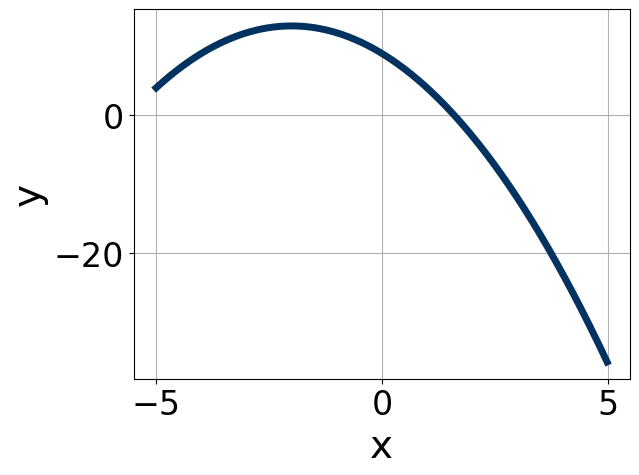
\includegraphics[width = 0.3\textwidth]{../Figures/quadraticEquationToGraphCopyAC.png}\item 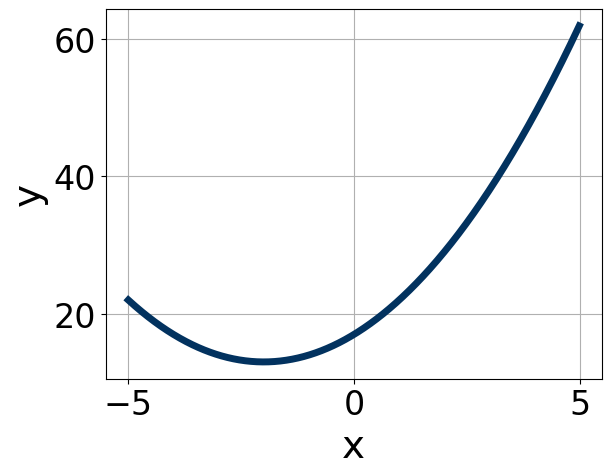
\includegraphics[width = 0.3\textwidth]{../Figures/quadraticEquationToGraphCopyBC.png}\item 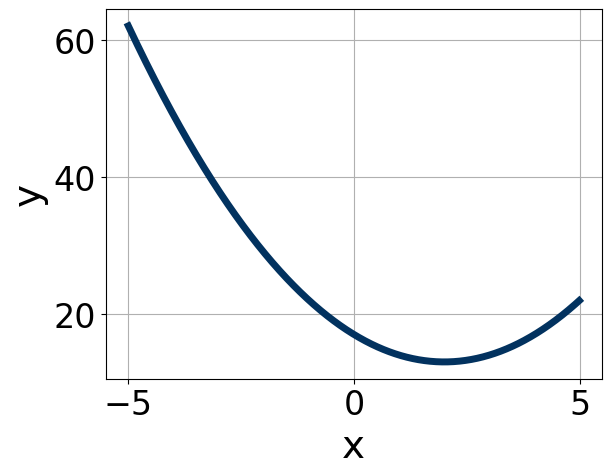
\includegraphics[width = 0.3\textwidth]{../Figures/quadraticEquationToGraphCopyCC.png}\item 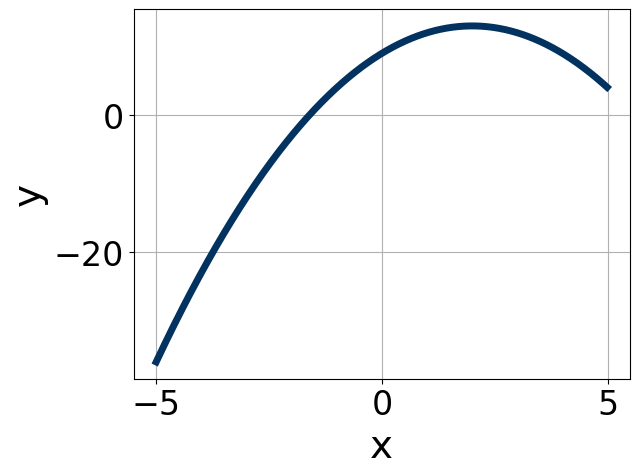
\includegraphics[width = 0.3\textwidth]{../Figures/quadraticEquationToGraphCopyDC.png}\end{multicols}\item None of the above.
\end{enumerate} }
\litem{
Graph the equation below.\[ f(x) = -(x-2)^2 - 14 \]\begin{enumerate}[label=\Alph*.]
\begin{multicols}{2}\item 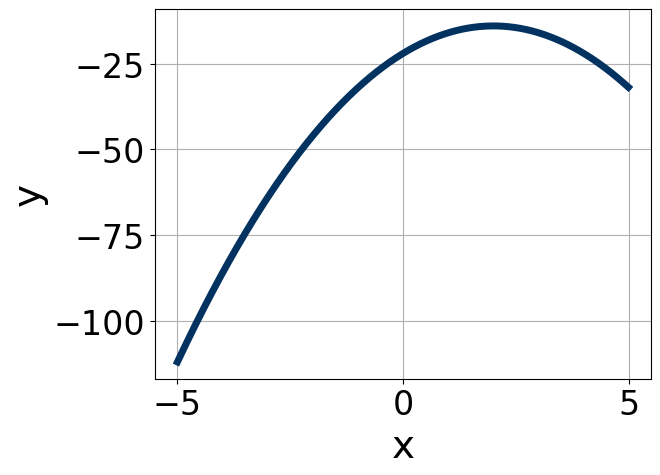
\includegraphics[width = 0.3\textwidth]{../Figures/quadraticEquationToGraphAC.png}\item 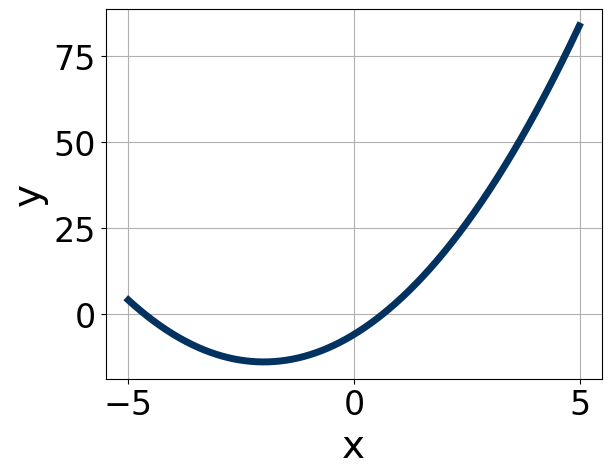
\includegraphics[width = 0.3\textwidth]{../Figures/quadraticEquationToGraphBC.png}\item 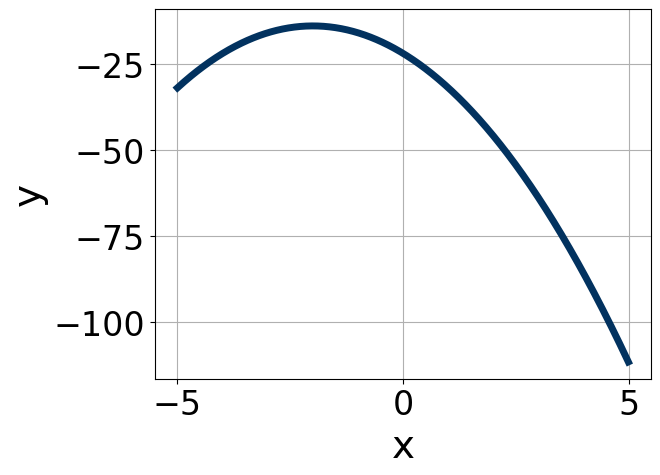
\includegraphics[width = 0.3\textwidth]{../Figures/quadraticEquationToGraphCC.png}\item 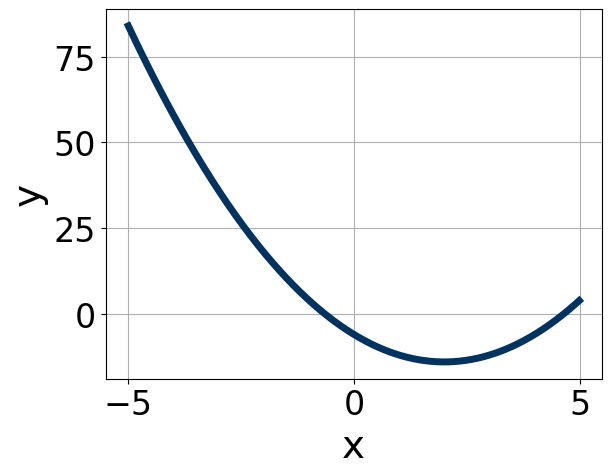
\includegraphics[width = 0.3\textwidth]{../Figures/quadraticEquationToGraphDC.png}\end{multicols}\item None of the above.
\end{enumerate} }
\litem{
Factor the quadratic below. Then, choose the intervals that contain the constants in the form $(ax+b)(cx+d); b \leq d.$\[ 24x^{2} +2 x -15 \]\begin{enumerate}[label=\Alph*.]
\item \( a \in [-0.33, 1.55], \hspace*{5mm} b \in [-22, -16], \hspace*{5mm} c \in [0.9, 1.7], \text{ and } \hspace*{5mm} d \in [17, 23] \)
\item \( a \in [7.04, 8.3], \hspace*{5mm} b \in [-6, 3], \hspace*{5mm} c \in [2.4, 5.6], \text{ and } \hspace*{5mm} d \in [-2, 8] \)
\item \( a \in [3.68, 4.18], \hspace*{5mm} b \in [-6, 3], \hspace*{5mm} c \in [3.1, 8.8], \text{ and } \hspace*{5mm} d \in [-2, 8] \)
\item \( a \in [1.79, 3.16], \hspace*{5mm} b \in [-6, 3], \hspace*{5mm} c \in [11.1, 15], \text{ and } \hspace*{5mm} d \in [-2, 8] \)
\item \( \text{None of the above.} \)

\end{enumerate} }
\litem{
Factor the quadratic below. Then, choose the intervals that contain the constants in the form $(ax+b)(cx+d); b \leq d.$\[ 24x^{2} -2 x -15 \]\begin{enumerate}[label=\Alph*.]
\item \( a \in [10.4, 12.3], \hspace*{5mm} b \in [-6, -1], \hspace*{5mm} c \in [1.13, 3], \text{ and } \hspace*{5mm} d \in [2, 14] \)
\item \( a \in [-1.5, 1.6], \hspace*{5mm} b \in [-23, -18], \hspace*{5mm} c \in [0.32, 1.03], \text{ and } \hspace*{5mm} d \in [12, 22] \)
\item \( a \in [1.8, 4.1], \hspace*{5mm} b \in [-6, -1], \hspace*{5mm} c \in [9.95, 13.55], \text{ and } \hspace*{5mm} d \in [2, 14] \)
\item \( a \in [5.4, 6.4], \hspace*{5mm} b \in [-6, -1], \hspace*{5mm} c \in [2.7, 5.28], \text{ and } \hspace*{5mm} d \in [2, 14] \)
\item \( \text{None of the above.} \)

\end{enumerate} }
\litem{
Write the equation of the graph presented below in the form $f(x)=ax^2+bx+c$, assuming  $a=1$ or $a=-1$. Then, choose the intervals that $a, b,$ and $c$ belong to.
\begin{center}
    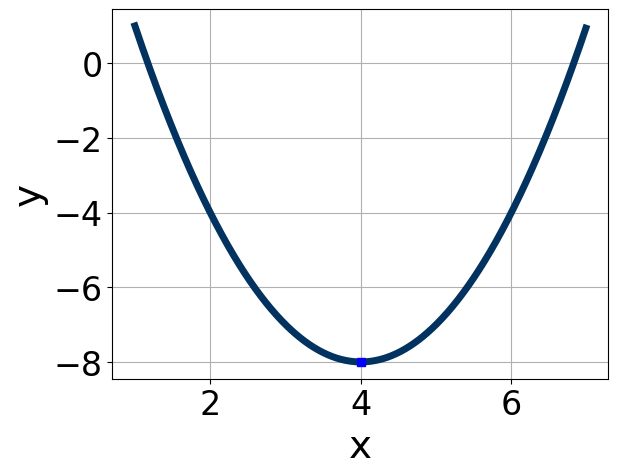
\includegraphics[width=0.5\textwidth]{../Figures/quadraticGraphToEquationCopyC.png}
\end{center}
\begin{enumerate}[label=\Alph*.]
\item \( a \in [1, 5], \hspace*{5mm} b \in [6, 9], \text{ and } \hspace*{5mm} c \in [22, 25] \)
\item \( a \in [1, 5], \hspace*{5mm} b \in [6, 9], \text{ and } \hspace*{5mm} c \in [6, 10] \)
\item \( a \in [-3, 0], \hspace*{5mm} b \in [6, 9], \text{ and } \hspace*{5mm} c \in [-28, -23] \)
\item \( a \in [-3, 0], \hspace*{5mm} b \in [-8, -6], \text{ and } \hspace*{5mm} c \in [-28, -23] \)
\item \( a \in [1, 5], \hspace*{5mm} b \in [-8, -6], \text{ and } \hspace*{5mm} c \in [6, 10] \)

\end{enumerate} }
\litem{
Solve the quadratic equation below. Then, choose the intervals that the solutions belong to, with $x_1 \leq x_2$ (if they exist).\[ 10x^{2} -12 x -2 = 0 \]\begin{enumerate}[label=\Alph*.]
\item \( x_1 \in [-1.62, -1.42] \text{ and } x_2 \in [12.5, 13.8] \)
\item \( x_1 \in [-14.51, -13.97] \text{ and } x_2 \in [15.1, 16.6] \)
\item \( x_1 \in [-0.21, 0.1] \text{ and } x_2 \in [0.5, 3.2] \)
\item \( x_1 \in [-1.47, -1.33] \text{ and } x_2 \in [-0.5, 0.3] \)
\item \( \text{There are no Real solutions.} \)

\end{enumerate} }
\litem{
Solve the quadratic equation below. Then, choose the intervals that the solutions $x_1$ and $x_2$ belong to, with $x_1 \leq x_2$.\[ 25x^{2} +10 x -24 = 0 \]\begin{enumerate}[label=\Alph*.]
\item \( x_1 \in [-4.3, -3.45] \text{ and } x_2 \in [0.22, 0.33] \)
\item \( x_1 \in [-30.14, -29.39] \text{ and } x_2 \in [19.97, 20.03] \)
\item \( x_1 \in [-6.56, -5.42] \text{ and } x_2 \in [0.09, 0.2] \)
\item \( x_1 \in [-0.74, -0.44] \text{ and } x_2 \in [1.54, 1.72] \)
\item \( x_1 \in [-1.48, -0.94] \text{ and } x_2 \in [0.78, 0.81] \)

\end{enumerate} }
\litem{
Solve the quadratic equation below. Then, choose the intervals that the solutions $x_1$ and $x_2$ belong to, with $x_1 \leq x_2$.\[ 25x^{2} +10 x -24 = 0 \]\begin{enumerate}[label=\Alph*.]
\item \( x_1 \in [-0.96, -0.54] \text{ and } x_2 \in [1.48, 1.68] \)
\item \( x_1 \in [-30.19, -29.58] \text{ and } x_2 \in [19.97, 20.16] \)
\item \( x_1 \in [-6.39, -5.98] \text{ and } x_2 \in [-0.05, 0.33] \)
\item \( x_1 \in [-1.21, -0.86] \text{ and } x_2 \in [0.76, 1.06] \)
\item \( x_1 \in [-3, -2.14] \text{ and } x_2 \in [0.37, 0.58] \)

\end{enumerate} }
\litem{
Solve the quadratic equation below. Then, choose the intervals that the solutions belong to, with $x_1 \leq x_2$ (if they exist).\[ 15x^{2} +10 x -2 = 0 \]\begin{enumerate}[label=\Alph*.]
\item \( x_1 \in [-0.39, 0.01] \text{ and } x_2 \in [0.44, 1.42] \)
\item \( x_1 \in [-0.91, -0.37] \text{ and } x_2 \in [-0.35, 0.29] \)
\item \( x_1 \in [-15.2, -15] \text{ and } x_2 \in [13.79, 15.29] \)
\item \( x_1 \in [-13.24, -11.89] \text{ and } x_2 \in [2.14, 3.09] \)
\item \( \text{There are no Real solutions.} \)

\end{enumerate} }
\end{enumerate}

\end{document}